\chapter{Estimativa financeira e otimização de custos}

Da maneira que o sistema foi projetado, cada trio de pontos de acesso dispostos no ambiente forma um módulo capaz de encontrar a posição do \emph{target} que se movimenta entre eles. Tendo isso em vista, compreende-se o modelo apresentado na figura a seguir, para o qual é formado o primeiro módulo com o trio de pontos de acesso desenhados em vermelho, abrangendo uma área aproximadamente circular de $\pi (\dfrac{r}{2})^2$ metros. Uma vez que o primeiro módulo é formado, nota-se que os próximos são compostos por dois nós do módulo adjacente mais um novo nó, como é o caso para as áreas verde e azul.

\begin{figure}[ht]
  \centering
    \caption{Modelo de mapeamento dos pontos de acesso}
    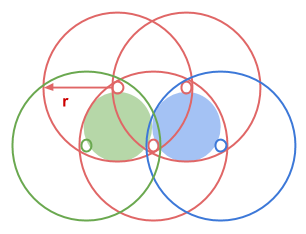
\includegraphics[scale=1]{estimativa-financeira}
	\centerline{\small{Fonte: autores}}
\end{figure}
\FloatBarrier

Assim, conclui-se que a quatidade de pontos de acesso necessários para cobrir uma área A é:

\begin{equation}
n = 3 + \dfrac{A - A_0}{A_0}, sendo A_0 = \pi (\dfrac{r}{2})^2
\end{equation}

Portanto, aplicando tal equacionamento para a reserva do Instituto Butantan, cuja cobertura completa seria de 80 hectares (A = 800.000m$^2$), e considerando o alcance medido para o dispositivo de r = 30m, temos que seria requisitada a aquisição de cerca de 1.130 \emph{SensorTags}, cujo preço unitário e de 29 dólares, finalmente estimando 32.770 dólares de custo inicial.

É notável que este gasto é substancialmente superior ao que seria consumido com os \emph{SensorTags} designados aos animais e com o controlador (RaspberryPi). Nesse sentido, é interessante tentar baratear o preço de cada ponto de acesso que, por não exigir a gama de sensores presente no \emph{SensorTag}, pode ter seu dispositivo simplificado - seria possível projetar e imprimir novas placas que contivessem somente antena Sub-1GHz e MCU 1350, cujo preço unitário é de 3,5 dólares. Também é relevante estudar se realmente seria interessante cobrir absolutamente toda a área da reserva ou se existem locais que não são visitados pelos animais monitorados.

Quanto ao custo de manutenção, deve-se levar em conta que a exposição ao ambiente de selva pode ser bastante hostil, tanto por acúmulo de sujeira, exposição a intempéries e possibilidade de extravio do dispositivo. Além disso, existiria troca da bateria em cada macaco pelo menos 3 ou 4 vezes por ano, cujo valor unitário é de 5 reais.